\chapter{Background}
\label{ch:background}

\renewcommand{\|}{\;|\;}

Distributed consensus systems have become a critical component of modern internet infrastructure, 
powering every major internet application at some level or another.
This chapter introduces the necessary background material for understanding and discussing these systems.
In addition, it introduces the pi-calculus, a formal language for describing concurrent processes,
which will be used to specify the Tendermint algorithm in Chapter \ref{ch:tendermint}.

\section{Replicated State Machine}

The most common paradigm for studying and implementing distributed consensus is that of the Replicated State Machine, 
wherein a \emph{deterministic} state machine is replicated across a set of processes, 
such that it functions as a single state machine despite the failure of some processes \cite{state_machine}.
The state machine is driven by a set of inputs, known as \emph{transactions}, 
where each transaction may or may not, depending on its validity, cause a state transition and return a result.
More formally, a transaction is an \emph{atomic} operation on a database, 
meaning it either completes or doesn't occur at all, 
and can't be left in an intermediate state \cite{transactions}
The state transition logic is governed by the state machine's state transition function,
which maps a transaction and the current state to a new state and a return value.
The state transition function is also sometimes referred to as \emph{application logic}.

It is the responsibility of the consensus protocol to order the transactions so that the resulting 
\emph{transaction log} is replicated exactly by every process.
Using a deterministic state transition function implies that 
every process will compute the same state given the same transaction log.

A summary of the replicated state machine architecture is given in Figure \ref{fig:replicated_state_machine}.

\begin{figure}[]
	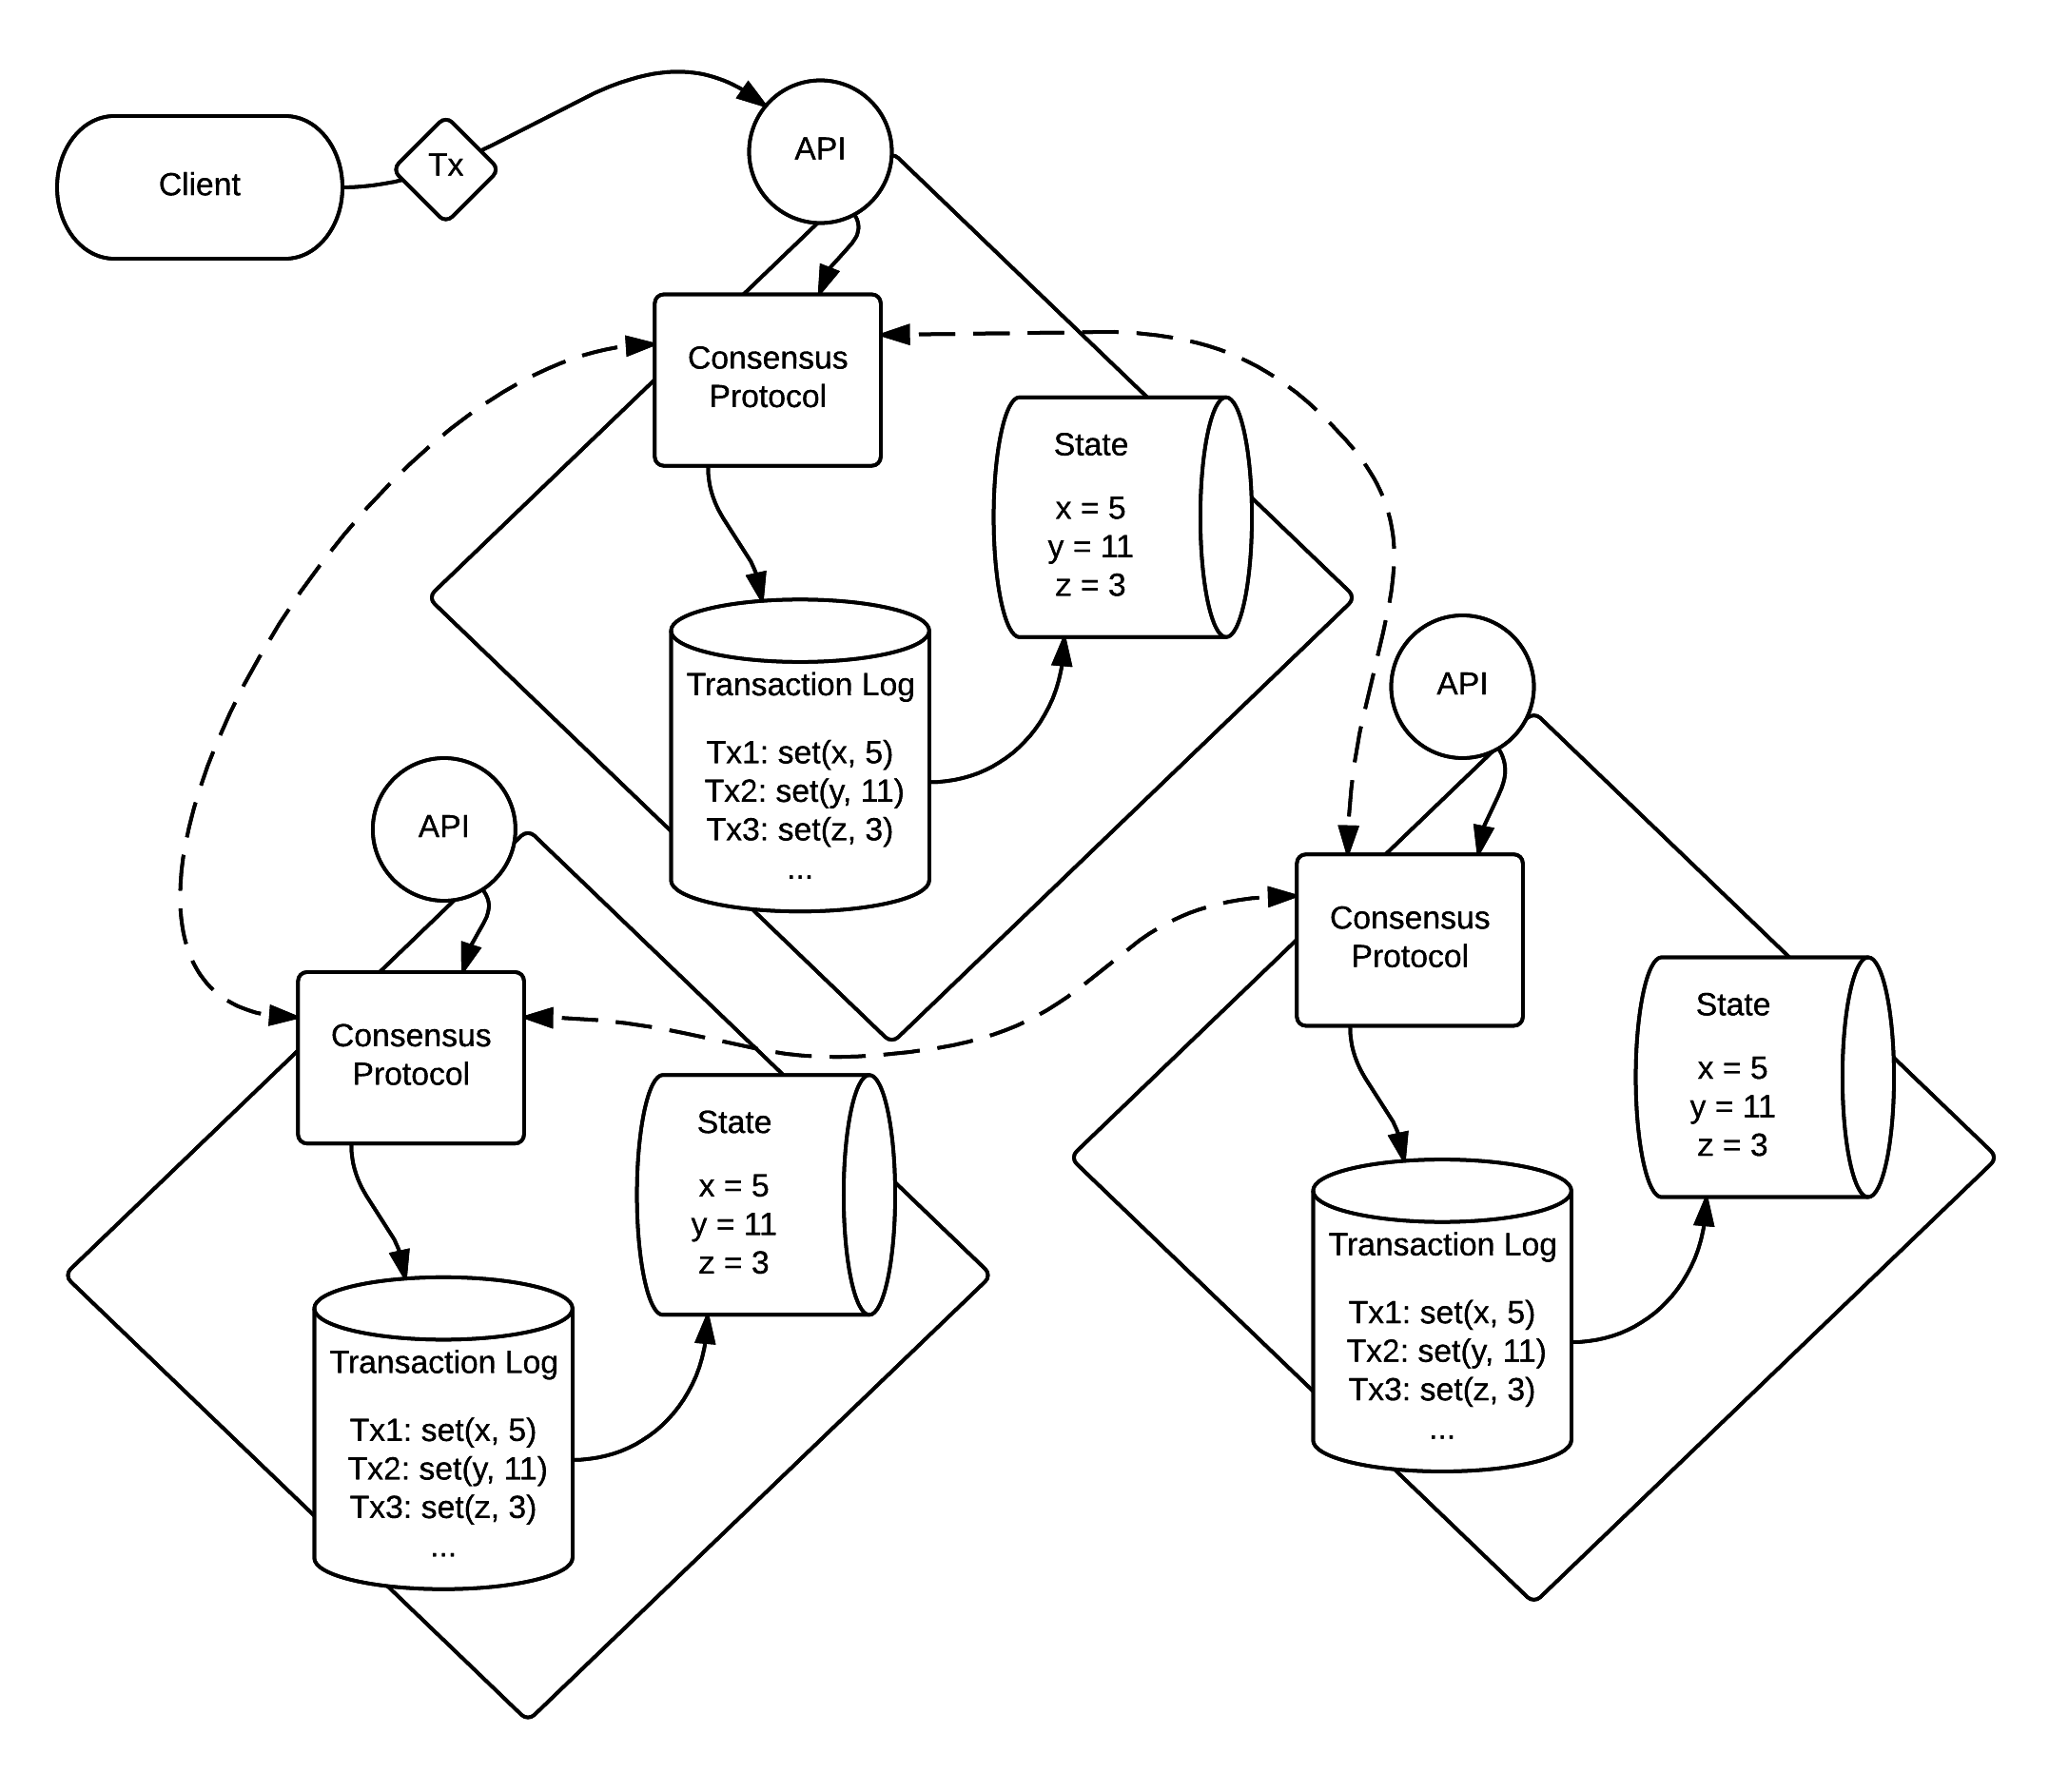
\includegraphics[width=\linewidth,height=\textheight,keepaspectratio]{figures/diagrams/state_machine.png}
    	\centering
	\caption[Overview of replicated state machine architecture]{
A replicated state machine replicates a transaction log and resulting state across multiple machines. 
Transactions are received from the client, 
run through the consensus protocol, 
ordered in the transaction log,
and executed against the state. 
In the figure, each diamond represents a single machine, 
with dotted lines representing communication between machines to carry out the consensus protocol for ordering transactions.}
	\label{fig:replicated_state_machine}
\end{figure}

Tendermint was motivated from the desire to create a general purpose, high-performance, secure, and robust replicated state machine.

\section{Asynchrony}

The purpose of a fault-tolerant replicated state machine is to co-ordinate 
a network of computers to stay in sync while providing a useful service, 
despite the presence of faults.

Staying in sync amounts to replicating the transaction log successfully; 
providing a useful service amounts to keeping the state machine available for new transactions.
These aspects of the system are traditionally known as \emph{safety} and \emph{liveness}, respectively.
Colloquially, safety means nothing bad happens; liveness means that something good eventually happens.
A violation of safety implies two or more valid, competing transaction logs.
Violating liveness implies an unresponsive network.

It is trivial to satisfy liveness by accepting all transactions. And it is trivial to satisfy safety by accepting none.
Hence, state machine replication algorithms can be seen to operate on a spectrum defined by these extremes.
Typically, processes require some threshold of received information from other processes before they commit a new transaction.
In synchronous environments, 
where we make assumptions about the maximum delay of network messages or the maximum speed of processor clocks,
 it is easy enough to take turns proposing new transactions, poll for a majority vote, 
and skip a proposer's turn if they don't propose within the bounds of the synchrony assumptions.

In asynchronous environments, where no such assumptions about network delays or processor speeds are warranted,
the trade-off is much more difficult to manage.
In fact, the so called FLP impossibility result demonstrates the 
impossibility of distributed consensus among deterministic asynchronous processes 
if even a single processes can crash\footnote{Prior to FLP, the distinction between sync/async wasn't as prominent}\cite{flp}.
The proof amounts to showing that, because processes can fail, 
there are valid executions of the protocol in which processes fail at the exact opportune times to prevent consensus.
Hence, we have no guarantee of consensus.

Typically, synchrony in a protocol is reflected by the use of timeouts to manage certain transitions.
In asynchronous environments, where messages can be arbitrarily delayed, relying on synchrony (timeouts) for safety
can lead to a fork in the transaction log.
Relying on synchrony to ensure liveness can cause the consensus to halt, and the service to become unresponsive.
The former case is usually considered more severe, as reconciling conflicting logs can be a daunting or impossible task. 

In practice, synchronous solutions are only used where the message latency is under 
extremely well defined control, for instance between controllers on an airplane \cite{},
or between datacenters that all posses a syncronized atomic clock \cite{spanner}.
Thus, while many efficient synchronous solutions exist,
the general unreliability of computer networks is too great a risk for them to be used in practice
without significant additional costs.

There are fundamentally two ways to overcome the FLP impossibility result.
The first is to use stronger synchrony assumptions - 
even rather weak assumptions are sufficient, 
for instance, that only eventually, 
crashed processes are suspected of crashing and correct ones are not \cite{chandra1996unreliable}.
Typically, this approach utilizes \emph{leaders}, 
which play a special co-ordinating role, 
and which can be skipped if they are suspected of being faulty after some timeout.
In practice, such leader-election mechanisms can be difficult to get right.

The second way to overcome FLP is to use non-determinism - 
include randomization elements such that
the probability of coming to consensus tends to $1$.
While clever, relying on randomization is typically much slower, 
though certain advanced cryptographic techniques have in recent years
achieved tremendous improvements in speed \cite{honeybadger}


\section{Broadcast and Consensus}

In order for a process to replicate its state on other processes, 
it must have access to basic communication primitives which allow it to disseminate, or deliver, information.
One of the most useful such primitives is \emph{reliable broadcast}.
Reliable broadcast (RBC) is a broadcast primitive satisfying \cite{rbc}, for message $m$:

\begin{itemize}
\item validity - if a correct process broadcasts $m$, it eventually delivers $m$
\item agreement - if a correct process delivers $m$, all correct processes eventually deliver $m$
\item integrity - $m$ is only delivered once, and only if broadcast by its sender
\end{itemize}

In essence, RBC enables a message to be eventually delivered on all correct processes.

Another, more useful primitive is \emph{atomic broadcast} (ABC), 
which satisfies RBC and an additional property:

\begin{itemize}
\item total order - if correct processes $p$ and $q$ deliver $m$ and $m'$, then $p$ delivers $m$ before $m'$ iff $q$ delivers $m$ before $m'$
\end{itemize}

In other words, atomic broadcast is a reliable broadcast where values are delivered in the same order on each host. 
Note this is exactly the problem of replicating a transaction log.
While colloquially, the problem may be referred to as consensus, 
the standard definition of the consensus primitive satisfies the following:
\begin{itemize}
\item termination - every correct process eventually decides
\item integrity - every correct process decides at most once
\item agreement - if one correct process decides $v1$ and another decides $v2$, then $v1=v2$
\item validity - if a correct process decides $v$, at least one process proposed $v$
\end{itemize}

Intuitively, consensus and ABC appear remarkably similar, 
with the critical difference that ABC is a continuous protocol,
whereas consensus expects to terminate.
That said, it is well known that each can be reduced to the other \cite{chandra1996unreliable}.
Consensus is easily reduced to ABC by deciding the first value to be atomically broadcast.
ABC can be reduced to consensus by running many instances of the consensus protocol, 
in sequence, 
though certain subtle considerations must be made, 
especially for handling Byzantine faults.
A complete description of the parameter space surrounding
the reduction of ABC to consensus remains an open topic of research.

Historically, despite the fact that most use cases actually require ABC,
the most widely adopted algorithm has been a consensus algorithm called Paxos, 
introduced, and proven correct, by Leslie Lamport in the 90s.
Paxos simultaneously empowered and confused the discipline of consensus science,
on the one hand by providing the first real-world, practical, fault-tolerant consensus algorithm,
and on the other by being so difficult to understand and explain.
Each implementation of the algorithm used its own unique bag of ad-hoc techniques
to build ABC from Paxos, making the ecosystem difficult to navigate, understand, and utilize.
Unfortunately, there was little work on improving the problem framing to make it more understandable.
though there were efforts to delineate solutions to the various difficulties \cite{chandra2007paxos}.

In 2013, Ongaro and Ousterhout published Raft \cite{raft},
a state machine replication algorithm whose motivating design goal was understandability.
Rather than starting from a consensus algorithm, and attempting to build what was needed (ABC),
the design of Raft considered first and foremost the transaction log,
and sought orthogonal components which could fit together to provide what is ultimately ABC,
though it is not described as such.

Paxos has been the staple consensus algorithm for industry, 
upon which the likes of Amazon \cite{dynamo}, Google \cite{chubby}, 
and others have built out highly available global internet services.
The Paxos consensus sits at the bottom of the application stack, 
providing a consistent interface to resource management and allocation, 
operating at much slower time scales than the highly-available applications facing the users.

Since its debut, however, Raft has seen tremendous adoption, especially in the open source community,
with implementations in virtually ever major language \cite{raft.github.io},
and use as the backbone in major projects, 
including CoreOs's distributed Linux distribution \cite{coreos_raft} 
and the open source time-series database InfluxDB \cite{influxdb,hashicorp_raft}.

Raft's major divergent design decisions from Paxos was to 
focus on the transaction-log first, rather than a single value,
in particular to allow a leader to persist in committing transactions until he goes down, 
at which point leadership election can kick in. 
In some ways, this is similar to the approach taken by blockchains, 
though the major advantage of blockchains is the ability to tolerate a different kind of fault.

\section{Byzantine Fault Tolerance}

Blockchains have been described as ``trust machines'' \cite{economist_blockchains} on account of the way they reduce counter party risk through the decentralization of responsibility over a shared database.
Bitcoin, in particular, is noted for its ability to withstand attacks and malicious behaviour by any of the participants. 
Traditionally, consensus protocols tolerant of malicious behaviour were known as Byzantine Fault Tolerant (BFT) consensus protocols.
The term Byzantine was used due to the similarity of the problem to that faced by generals of the Byzantine army attempting to co-ordinate themselves to attack Rome using only messengers,
where one of the generals may be a traitor \cite{lamport1982byzantine}.

In a crash fault, a process simply halts. In a Byzantine fault, it can behave arbitrarily.
Crash faults are easier to handle, as no process can \emph{lie} to another process.
Systems which only tolerate crash faults can operate via simple majority rule, 
and therefore typically tolerate simultaneous failure of up to half of the system.
If the number of failures the system can tolerate is $f$, such systems must have at least $2f+1$ processes.

Byzantine failures are more complicated. In a system of $2f+1$ processes, if $f$ are Byzantine, 
they can co-ordinate to say arbitrary things to the other $f+1$ processes.
For instance, suppose we are trying to agree on the value of a single bit, 
and $f=1$, so we have $N=3$ processes, $A$, $B$, and $C$, where $C$ is Byzantine, as in Figure \ref{fig:byzantine}.
$C$ can tell $A$ that the value is $0$ and tell $B$ that it's $1$. 
If $A$ agrees that its $0$, and $B$ agrees that its $1$, then they will both think they have a majority and commit, 
thereby violating the safety condition.
Hence, the upper bound on faults tolerated by a Byzantine system is strictly lower than a non-Byzantine one.

\begin{figure}[]
	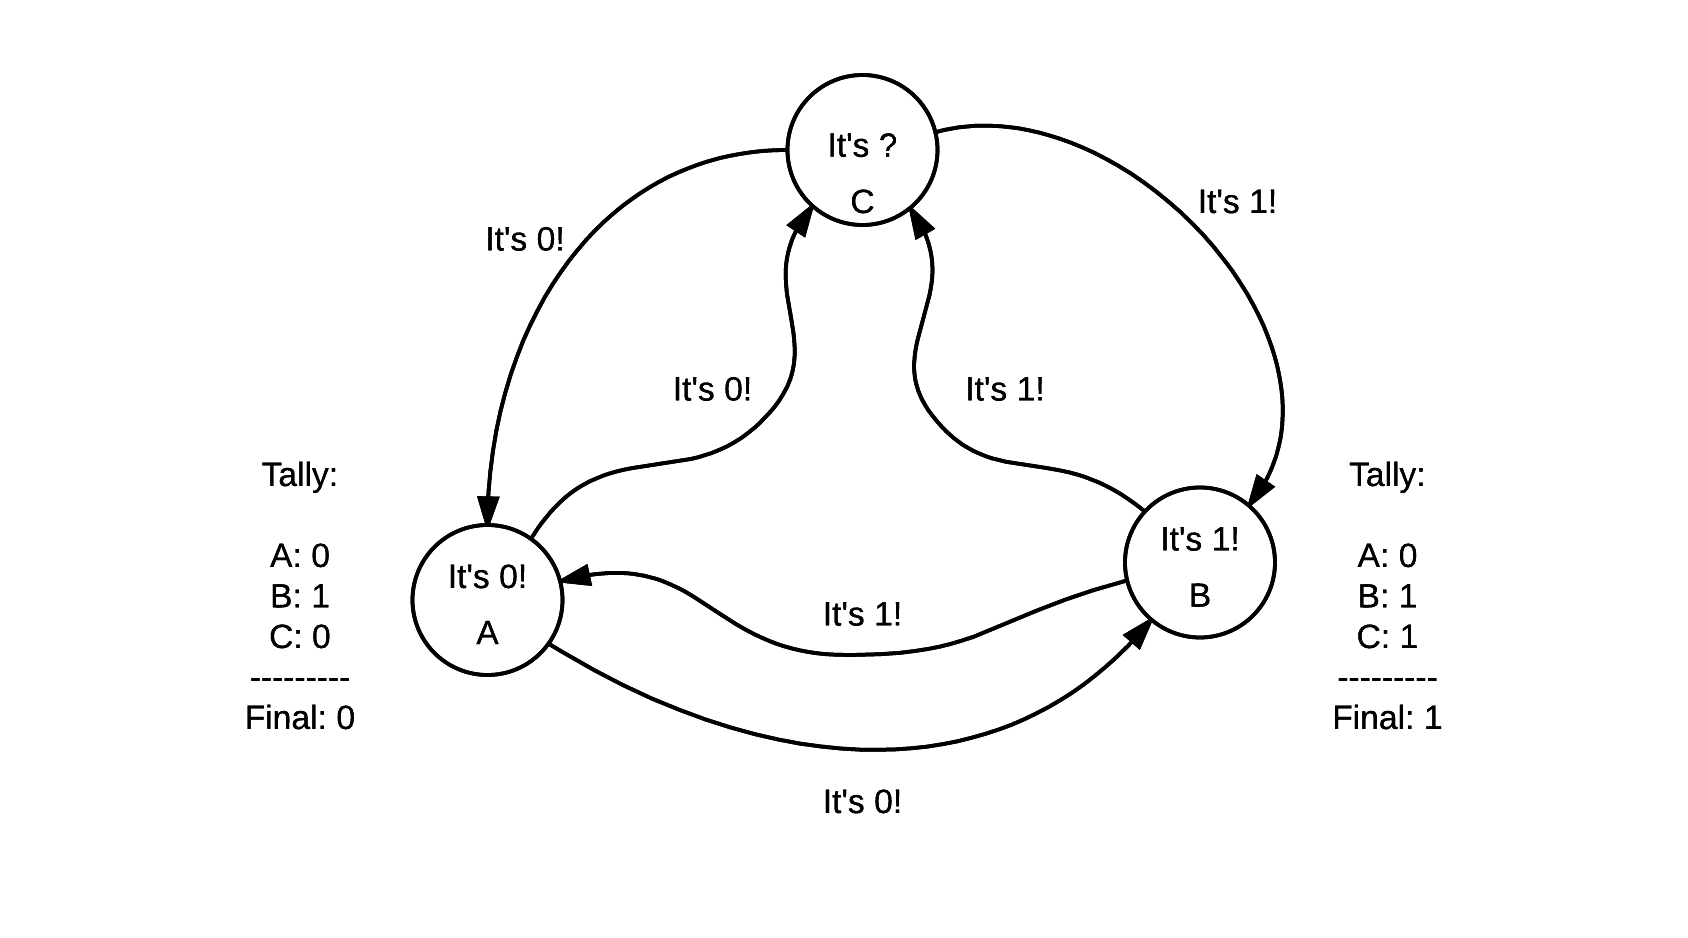
\includegraphics[width=\linewidth,height=\textheight,keepaspectratio]{figures/diagrams/byzantine.png}
    	\centering
	\caption[Byzantine processes tell lies]{
A Byzantine process, C, tells A one thing and B another, causing them to come to different conclusions about the network.
Here, simple majority vote results in a violation of safety due to only a single Byzantine process.}
	\label{fig:byzantine}
\end{figure}


In fact, it can be shown that the upper limit on $f$ for Byzantine faults is $f < N/3$ \cite{pease1980reaching}.
Thus, to tolerate a single Byzantine process, we require at least $N=4$. 
Then the faulty process can't split the vote the way it was able to when $N=3$.

In 1999, Castro and Liskov published Practical Byzantine Fault Tolerance \cite{pbft}, or \emph{PBFT}, 
which provided the first optimal Byzantine fault tolerant algorithm in asynchronous networks.
It set a new precedent for the practicality of Byzantine fault tolerance in industrial systems by being capable 
of processing tens of thousands of transactions per second.
Despite this success, Byzantine fault tolerance was still considered expensive and largely unnecessary, 
and the most popular implementation was difficult to build on top of \cite{ppbft}.
Hence, despite a resurgence in academic interest, including numerous improved variations \cite{yin2003separating, kotla2007zyzzyva}
not much progress was made in the way of implementations and deployment.
Furthermore, PBFT provides no guarantees if a third or more of the network co-ordinates to violate safety.

\section{Cryptography, Trust, and Economics}

Fundamentally, fault tolerance is a problem derriving from a lack of trust - 
an inability to know how some process will behave.
Formally, trust might be defined information theoretically as a means
for reducing the entropy of one's model of the world - 
to trust someone is to optimistically reduce one's uncertainty about the world,
enabling more focused attention on higher order forms of organization.

Cryptographic primitives are also fundamentally related to the problem of trust,
and may similarly be defined as mechanisms which allow for a massive reduction in entropy -
succesfully authenticating a cryptographic function collapses a distribution 
over possible outcomes to a single, or in some cases a small number, of outcomes.

It is well known that civilizations that have greater forms of institutional trust,
such as the rule-of-law, 
have higher productivity and more vibrant economies \cite{trust}.
The result makes intuitive sense, as being able to trust more about an interaction 
reduces the space of possible outcomes that need to be actively modelled,
making it easier to co-ordinate.
Unfortunately, it is becoming increasingly difficult to evaluate the trustworthiness 
of modern institutions as their complexity has skyrocketed in recent decades,
increasing the likelihood that the certainty they allegdly provide is an illusion.

Fortunately, cryptography can form the basis for new institutions of trust in society 
which may dramatically improve the capacity for human co-ordination at global scale on account
of reduced risk of fraudulent and/or unaccountable activity.
Of particular interest is the importance of cryptographic primitives in BFT algorithms,
both for authentication and for seeding non-determinism.

Most interestingly, economic mechanisms may also serve as means for reducing entropy,
in so far as economic agents can be incentivized - 
which is to say be made more likely to execute a particular behaviour.
In fact, Bitcoin's great insight was that cryptographic primitives could be used in
conjuction with economic incentives to sufficiently reduce the entropy of a public consensus network
to achieve secure replication of state.

A more formal investigation of the information theoretic grounds of trust, cryptography,
consensus, and economics, and in particular their inter-relationship, remains for future work.

\section{Blockchain}

A blockchain is, at heart, an integrity-focused approach to Byzantine Fault Tolerant Atomic Broadcast.
The Bitcoin blockchain, for instance, uses a combination of economics and cryptographic randomization 
to provide a strong probabilistic gaurantee that safety will not be violated, 
given a weak synchrony condition, namely, 
that blocks are gossipped much more rapidly than they are found via the partial-hash collision lottery.
In practice, however, it is well known that Bitcoin's security guarantees are vulnerable to a number 
of subtle attacks \cite{selfish_mining,block_witholding}.

The blockchain gets its name from the two key optimizations it employs in solving ABC.
The first is that it groups transactions in blocks in order to amortize the high commit latency 
(on the order of ten minutes) over many transactions.
The second is to link blocks via cryptographic hashes into an immutable chain,
such that is easy to verify the historical record.
Both optimizations are natural improvements to a naiive BFT-ABC,
the former improving performance, the latter improving tolerance to certain kinds 
of difficult to model Byzantine faults.

Over the last few years, it has become common to ``blockchainize'' consensus algorithms,
that is, to adopt them to ABC using the blockchain paradigm of hash-linked transaction batches.
To the author's knowledge, Tendermint was the first such proposal, 
upgrading a well known BFT algorithm from the late 80s \cite{dls},
though it has since evolved to a consensus algorithm of its own.
It has been followed by IBM, which upgraded PBFT to a blockchain \cite{obc_},
and by JP Morgan, which upgraded a BFT version of Raft \cite{juno}.

\section{Process Calculus}

Distributed systems, where pieces of the system execute concurrently with one another,
are notorious for being difficult to design, build, and debug.
They are further difficult to formally verify, 
as most techniques for formal verification, and in fact the very foundations of computer science,
have been specifically developed with sequential computation in mind.

Process calculi are a family of models introduced 
to provide a formal basis for concurrent computation.
The most popular calculus, the Comunicating Sequential Processes (CSP) \cite{csp}
forms the theoretical foundation for many modern programming languages which 
include concurrency primitives in the language design \cite{csp_go}.

In the 80s, Robin Milner introduced the Calculus of Communicating Systems (CCS), 
designed to be a concurrent analog of the sequential lambda calculus that underlies most functional programming languages.
While the lambda calculus has function application as its basic unit of computation,
CCS uses communication between two concurrent processes over a shared channel as its basic operational primitive.
A more general form of CCS, the $\pi$-calculus, 
enables mobility in the communication graph between processes, 
such that the channels of communication can themselves be passed along other channels,
thereby blurring the distinction between data, variables, and channels.
The result is a coherent, minimalistic model of computation more powerful than its sequential predecessors.

The $\pi$-calculus has proven to be a highly effective tool for the study of concurrent systems,
with applications from business process management \cite{pi_biz} to cellular biology \cite{stochastic_pi}.
The remarkably simple notation simplifies the description of concurrent protocols.
Furthermore, the well known equivalence between computation and logic \cite{curry_howard} enables
logical systems to be defined complementary to the various process calculi,
providing formal means to discuss and verify the properties of systems specified in an appropriate calculus.

While we use the $\pi$-calculus to specify the Tendermint algorithm, 
we leave use of an associated formal logic, and the corresponding verification of properties, to future work.

The grammar of the $\pi$-calculus, in Backus-Naur form, is as follows:


\begin{center}
	\begin{tabular}{l }
		{$\!\begin{aligned}
			P & := & 0  & & \text{ \emph{void}}\\
			    & \; \| & P \| P  & & \text{ \emph{par}} \\
			    & \; \| & \alpha.P  & & \text{ \emph{guard}} \\
			    & \; \| & \alpha.P  + \alpha.P & & \text{ \emph{guarded-choice}} \\
			    & \; \| & (\nu x) P & & \text{ \emph{fresh}}\\ \\

			\alpha & := & \tau & & \text{ \emph{null}} \\
			    & \; \| & x!(y) & & \text{ \emph{send}} \\
			    & \; \| & x?(y) & & \text{ \emph{receive}}\\
		\end{aligned}$} \\ 
	\end{tabular}
\end{center}

Each grammatical rule is labelled with a reference to its functional meaning.
In essence, a process may be the empty process, $0$, 
or it may be two processes running concurrently, $P \| P$.
A guarded processes, $\alpha.P$, only allows process $P$ to execute after an action, $\alpha$,
has occured.
The action can be a null action, $\tau$, or it can be the sending, $x!(y)$, 
or receiving, $x?(y)$, of $y$ along $x$.
Guarded choice injects non-determinism into the operation of the calculus, 
such that the processes $\alpha.P + \beta.Q$ will non-deterministically execute
$\alpha$ or $\beta$, and then run $P$ or $Q$, respectively.
Finally, a new channel, $x$, can be created via $(\nu x) P$, such that $x$ is only accessible in $P$.

A structural congruence on processes is defined as the largest relation satisfying


Structural congruence permits certain forms of re-arranging of a process term that will still yield the same process.
On the other hand, an operational semantics defines the actual non-reversible computational steps that a process may execute.
Effectively, the only relevant operation is communication, known as the \emph{comm} rule:


Now, given a $\pi$-calculus process, we can follow its execution by applying the comm rule.
For instance, the process


Applied - functions, other notation, broadcast, etc.

Logic ...


\section{The Need For Tendermint}

The success of Bitcoin and its derivatives, especially Ethereum, and their promise of secure, autonomous, distributed, fault-tolerant execution of arbitrary code has caused virtually every major financial institution on the planet to become interested in the blockchain phenomenon. 
In particular, there has emerged an understanding of two forms of the technology:
On the one hand are the public blockchains, known affectionately as the Big Bad Public Blockchains or BBPBs, 
whose protocols are dominated by in-built economic incentives bootstrapped by a native currency.
On the other are so called private blockchains, which might more accurately be called ``consortia blockchains'',
and which are effectively improvements on traditional consensus and BFT algorithms through the use of hash trees, digital signatures, 
peer-to-peer networking, and enhanced accountability.

As the infrastructure of our societies continues to decentralize, and as the nature of business becomes more inter-organizational,
there is increasing need for a transparent, accountable, high performance BFT system, which can support applications from finance to domain registration to electronic voting,
and which comes equipped with advanced mechanisms for governance and evolution into the future.
Tendermint is that solution, optimized for consortia, or inter-organizational logic, but flexible enough to accommodate anyone from private enterprise to global currency,
and high-performance enough to compete with the major, non-BFT, consensus solutions available today, such as etcd, consul, and zookeeper, while providing greater resilience, security guarantees, and flexibility to application developers.

A more comprehensive discussion of consensus science and related algorithms is reserved for Chapter \ref{ch:related}

